\chapter{Introduction}

\graphicspath{{Chapter1/figures/}}

Introduce:

-- sensemaking and explain why supporting it is important and challenging

-- vis and its capability of supporting sensemaking

\section{Research Problem and Approach}
\subsection{Problem}
Overall, this research aims to \emph{examine how to support users making sense of their problems}. 

Introduce analytic provenance and justify why it is a potential approach to support sensemaking.

Summarize the process in which analytic provenance provides support to sensemaking.

%Pirolli and Card~\cite{Pirolli2005} describe sensemaking as a process consisting of two loops: the \emph{foraging loop}, which involves searching, extracting and organizing information; and the \emph{sensemaking loop}, which involves building schemas, generating and testing hypotheses, and presenting the outcome. Schematization plays an important role in this model: connecting the foraging loop and the sensemaking loop. It is a crucial step in converting raw evidence to rational explanations. Pirolli and Card suggest that the schematization process should be supported by a computer-based tool that organizes raw evidence into small-scale stories about typical topics or in answer to typical questions (e.g., who, what, when, where, why, how). This suggestion is aligned with a recent empirical study by Kang, Görg and John Stasko~\cite{Kang2011}. It shows that all of the participants who performed the sensemaking task well spent considerable time and effort in \emph{organizing their collected information}. Their organizational schemes were flexible: a \emph{timeline} of related events, a \emph{map} connecting locations that a person has been to, and a \emph{diagram} showing relationships among suspicious targets.

%One approach to provide such support is through \textbf{analytic provenance} -- an area of research focusing on understanding a user's reasoning process through the study of their interactions with a visualization tool~\cite{North2011}. More specifically, during the process in which a user solves a sensemaking task using a visualization tool, their interactions and discoveries -- we refer to both of them as \emph{provenance data} -- are captured and visualized to provide support back to the sensemaking process itself as summarized in Figure~\ref{fig:workflow}. 

\begin{figure}[!htb]
	\centering
	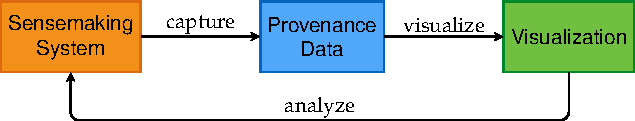
\includegraphics{workflow}
	\caption{A pipeline of supporting sensemaking through analytic provenance. During the process in which a user solves a sensemaking task using a visualization tool, their interactions and discoveries -- we refer to both of them as \emph{provenance data} -- are captured, visualized and analyzed to provide support back to the sensemaking process.}
	\label{fig:workflow}
\end{figure}

In this thesis, we focus on the \textbf{visualization} part of that process:
\begin{center}
	\strong{How to design interactive visualizations of provenance data \\to support sensemaking?}
\end{center}

\subsection{Approach}
%The research is driven by enabling users to discover the answers to the aforementioned questions (who, what, when, where, why, how) of the captured provenance data.
%\begin{enumerate}
%	\item \strong{when?} this is to help users to analyze the \textbf{temporal} relationship of their provenance data. Current timeline visualization has these limitations
%	\begin{itemize}
%		\item no or very simple layout which is cluttered and space-inefficient
%		\item designed for presenting a known story rather than interactively constructing a hidden one
%	\end{itemize} 
%	\item \strong{who/what?} grouping information related to a person or a topic together allows users to have a better understanding of their provenance data. It is more useful if such \textbf{thematic} information can be visualized together with the temporal information. Currently, this is still an open challenge. These three principles of Gestalt's laws of grouping are typically employed to visualize set relations on a timeline:
%	\begin{itemize}
%		\item similarity: use colors or shapes to indicate sets -- not powerful 
%		\item proximity: not space-efficient
%		\item uniform connectedness: cluttered
%	\end{itemize} 
%	\item \strong{why?} discover and visualize \textbf{semantic/causal} relationships of user's provenance data is a step towards answering this question. After a long period of working on the sensemaking task, the user may get lost. At a low level, they may fail to find the information they discovered before. At a higher level, they may not know where they are in the context of the overall task, and may not know where to continue. Existing visualizations do not fully support users to overcome this \emph{disorientation} problem.
%\end{enumerate}
%
%We choose not to address the \textbf{where} question because spatial information is not always available and relevant to the task. If locations are named, we can consider them as \emph{themes} and use the methods for \textbf{who/what} questions to analyze them. We do not address the \textbf{how} question; however, combining the answers to \textbf{when} and \textbf{who/what} questions may help improve understanding about it.

%We take a user-centered design approach in developing the solutions to the three aforementioned questions. For each question, we elicit the design requirements either by conducting a user study or drawing from the literature. Visual encoding and interaction are designed to meet those requirements and are implemented into a working prototype. Finally, an empirical study is conducted to validate if the tool supports users as intended.  
%
%The analytic provenance approach that we take is general; however, we need to choose specific domains/tasks to demonstrate its application. Sensemaking does not only happen when using a visualization system to solve a ``serious'' intelligence analysis task. Actually, it often happens in our life such as when using a web browser to find information to select the most suitable smartwatch to buy. Therefore, to demonstrate the wide application of our visualization techniques, we target both intelligence analysis tasks using a visualization system and everyday sensemaking tasks using a web browser.

Two types of provenance data:
\begin{itemize}
	\item user thinking: typically from user notes, high user effort, rich semantics 
	\item user interaction: automatic capture, no user effort, poor semantics
\end{itemize}

Two types of relationship in the sensemaking process that provenance data may help to reveal:
\begin{itemize}
	\item temporal: understand the process ('how')
	\item logical: understand the rationale ('why')
\end{itemize}

To address the research problem, we take an incremental approach, progressing from the least impact (high user effort to understand the process) towards the most impact (no user effort to understand the rationale).

Two domains to demonstrate:
\begin{itemize}
	\item intelligence analysis: rigorous sensemaking problems
	\item everyday sensemaking with web browser: popular, high demands
\end{itemize}
\section{Thesis Contributions}
%Chapter 2 provides an overview of sensemaking, visualization and analytic provenance.
%
%Chapter 3 reviews related work of visualizing provenance data to support sensemaking.
%
%Chapter 4 presents a compact yet aesthetically pleasing timeline visualization technique that enables users to interactively construct a temporal schema from provenance data.
%
%Chapter 5 extends Chapter 4 to present a timeline visualization technique that can effectively show both temporal and set information of provenance data. This technique can also be used for more general data.
%
%Chapter 6 discusses the requirements, design, implementation and evaluation of a visualization system that enables users to have an overview of their sensemaking process, to organize their provenance data in such a way that aids their understanding about the task, and to communicate their findings at different levels of granularity.
%
%Chapter 7 describes a general approach that combines analytic provenance and visualization to shorten the transcription and coding steps in qualitative data analysis, and a tool to demonstrate its application.
%
%Finally, Chapter 8 concludes the thesis with a discussion on its contributions and future research directions triggered from this work.

Towards the overall goal of supporting users in their sensemaking processes, this thesis contributes
\begin{itemize}
	\item a compact yet aesthetically pleasing timeline visualization technique that enables users to explore and construct temporal narratives from user annotations.
	\item a novel timeline visualization technique that enables users to explore more complex temporal narratives by effectively showing both temporal and thematic information. %This technique can also be used for more general data.
	\item a novel application of analytic provenance approach to qualitative data analysis that enables researchers to understand the users' sensemaking processes and a visualization tool to demonstrate its success.% They can be applied to qualitative data analysis.  general approach that combines analytic provenance and visualization to shorten the transcription and coding steps in qualitative data analysis, and a tool to demonstrate its application.
	\item a light-weight visualization tool (as a browser plugin) system that enables users to see their logical sensemaking processes, to organize the relevant information in such a way that aids their understanding about their problems, and to communicate their findings at different levels of granularity.
\end{itemize}

%mention the papers and co-authors' contributions here
%mention also old SenseMap paper, Rick paper, research agenda?
%list of publication in a separate page

\section{Thesis Outline} 

\begin{figure}[!htb]
	\centering
	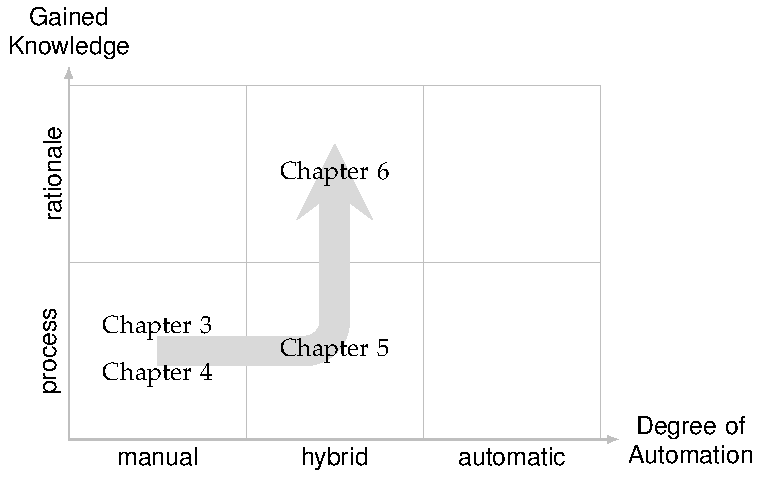
\includegraphics{work}
	\caption{Positioning upcoming chapters into the analysis of the degree of automation and the gained knowledge.}
	\label{fig:work}
\end{figure}

%\begin{figure}[!htb]
%	\centering
%	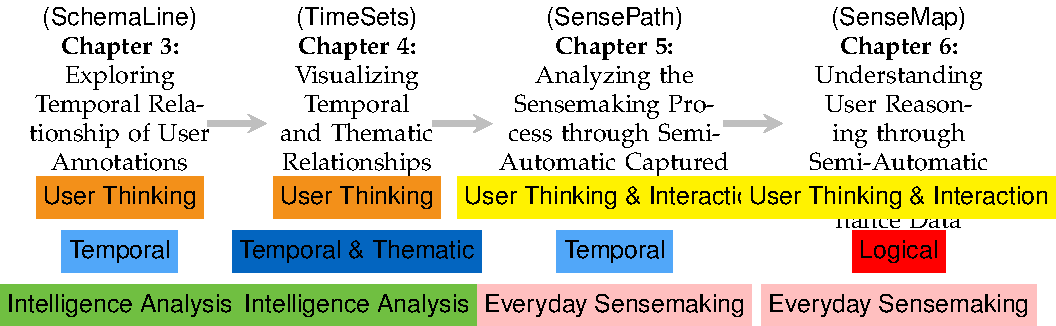
\includegraphics{story}
%	\caption{Summary of upcoming chapters.}
%	\label{fig:story}
%\end{figure}

%Chapter 2 provides an overview of sensemaking, visualization and analytic provenance.
%
%Chapter 3 reviews related work of visualizing provenance data to support sensemaking.
%
%Chapter 4 presents the design, layout and evaluation of a timeline visualization technique that is designed to support sensemaking.
%
%Chapter 5 extends the timeline visualization in Chapter 4 to include thematic information.
%
%Chapter 6 discusses the requirements, design, implementation and evaluation of SenseMap -- a browser plugin that enables users to collect, curate and communicate their findings.
%
%Chapter 7 describes 
%
%Finally Chapter 8 concludes the thesis with a discussion on its contributions and future research directions triggered from this work.
